\documentclass{IEEEtran}

\usepackage{amsmath}
\usepackage{graphicx}

\title{Assignment I - ICSE 10 2018 - Q9(a)}
\author{Kartheek Tammana}

\begin{document}
\maketitle

Equation for interest $I$ on a reccuring deposit is:

\begin{equation}
I = \frac{P \cdot n(n+1) \cdot r}{12 \cdot 2 \cdot 100}
\end{equation}

Where $P$ is the monthly deposit (in rupees), $n$ is total time (in months), and $r$ is percentage
annual interest.

We are given $I = 5550$, $P=1000$, and $r=10$. Substituting, we get

\begin{gather*}
    5550 = \frac{1000 \cdot n(n+1) \cdot 10}{12 \cdot 2 \cdot 100} \\ \\
    n(n+1) = \frac{5550 \cdot 2400}{10000} = 1332 = 36 \cdot 37
\end{gather*}

Solving the quadratic, we get $n=36$ or $n=-37$. Discarding the negative solution, we get that the
time of maturity is 36 months, or 3 years. \\ \\
We can verify this answer by graphing the interest as a function of time, i.e.,
\begin{equation}
y = \frac{5550 \cdot x(x+1) \cdot 10}{12 \cdot 2 \cdot 100}
\end{equation}
along with the interest at time of maturity $y=5550$, and checking for the point of intersection,
where $y$ is the interest in rupees, and $x$ is time in months.
\centering
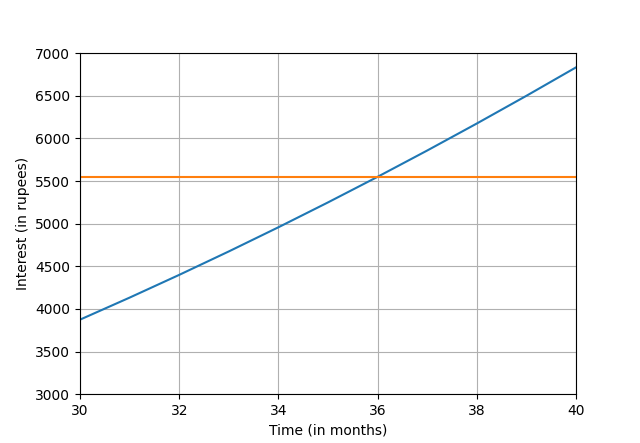
\includegraphics[width=0.75\columnwidth]{./figs/fig.png}
\end{document}
